\section{Thiết kế cơ chế phát hiện}
\label{sec:methodology}

\subsection{Tổng quan cách tiếp cận}
Cơ chế phát hiện leo thang đặc quyền được thiết kế theo nguyên tắc
\emph{huấn luyện-rồi-phục-vụ}: lõi phát hiện bất thường syscall (SyscallAD) kế thừa
thiết kế của công trình tham chiếu DeSFAM~\cite{desfam_original}, với bộ dữ liệu,
định nghĩa đặc trưng và giao thức đánh giá được cố định để có thể đối chiếu trực
tiếp với số liệu công bố. Thành phần phục vụ trực tiếp giám sát theo namespace
(tenant) trên Kubernetes nhằm kiểm chứng tính khả thi triển khai của cơ chế.

\subsection{Kiến trúc tổng thể}
Hình~\ref{fig:arch} mô tả kiến trúc ba mô-đun (giai đoạn) theo công trình tham
chiếu: (1) lập hồ sơ/danh sách truy cập syscall lai; (2) phát hiện bất thường
\emph{SyscallAD}; (3) thực thi thích ứng/phản ứng. \textbf{Trọng tâm của chuyên đề
là mô-đun SyscallAD (Giai đoạn~2)}; đây cũng là phần được hiện thực hóa và đánh giá
trọn vẹn. Hai mô-đun còn lại chỉ được \emph{điểm qua}: Giai đoạn~1 (sinh danh sách
truy cập tĩnh+động, hồ sơ seccomp, lọc theo CVE) được tóm tắt ở
Mục~\ref{sec:related} và không được hiện thực hóa lại; ở Giai đoạn~3 chuyên đề chỉ
tận dụng lớp thu thập/cảnh báo (Tetragon ghi nhật ký, phát cảnh báo), còn cơ chế
chấm điểm rủi ro (ánh xạ MITRE ATT\&CK) và chặn nội tuyến trong nhân bằng eBPF/LSM
được nêu là hướng mở rộng chứ không thuộc phạm vi nghiên cứu chính.

\begin{figure}[htbp]
  \centering
  
\includegraphics[width=\linewidth]{figures/desfam-architecture}
  \caption{Kiến trúc cơ chế phát hiện (kế thừa thiết kế tham chiếu DeSFAM): cảm
           biến syscall (eBPF/Tetragon) giám sát theo namespace $\to$ trích đặc
           trưng theo cửa sổ trượt $\to$ SyscallAD (VAE + iForest) $\to$ chấm điểm
           rủi ro và phản ứng. Mũi tên ngoại tuyến: huấn luyện trên DongTing; mũi
           tên trực tuyến: phục vụ trên multi-tenant Kubernetes.}
  \label{fig:arch}
\end{figure}

\subsection{Dữ liệu và tiền xử lý}
Nguồn dữ liệu ngoại tuyến là bản phát hành DongTing~\cite{ref26_dongtingdataset}
($18{,}9$ nghìn chuỗi được gán nhãn, các tệp \texttt{.log} kèm bảng phân chia
\texttt{Baseline.xlsx}). Chuỗi bình thường lưu dưới dạng \emph{ID syscall} phân
tách bằng dấu gạch đứng; chuỗi tấn công lưu dưới dạng \emph{tên syscall}. Chúng
tôi dùng bảng \texttt{syscall\_64.tbl} (x86-64, bỏ các dòng ABI x32) để ánh xạ
tên\,$\leftrightarrow$\,ID nhất quán. Phân chia theo bộ dữ liệu:
\texttt{DTDS-train} / \texttt{DTDS-validation} / \texttt{DTDS-test}.

\paragraph{Bảng chữ cái cảm biến (sensor alphabet).} Đây là quyết định thiết kế
\emph{then chốt} để tái lập thành công khâu triển khai trực tiếp. Chính sách truy
vết trực tiếp của Tetragon chỉ phát ra \textbf{23 syscall liên quan an ninh}
(\texttt{execve}, \texttt{clone}, \texttt{setuid/setgid/capset}, \texttt{openat},
\texttt{unlinkat}, \texttt{renameat2}, \texttt{mount}, \texttt{unshare},
\texttt{setns}, \texttt{pivot\_root}, \texttt{socket}, \texttt{connect},
\texttt{bind}, \texttt{mprotect}, \texttt{mmap}, \texttt{prctl},
\texttt{memfd\_create}, \texttt{splice}, \texttt{ptrace},
\texttt{init/finit\_module}, \texttt{bpf}---\emph{không} gồm
read/write/close/futex). Do đó khâu huấn luyện cũng lọc DongTing về đúng tập này
\emph{trước} khi cắt cửa sổ, để huấn luyện và phục vụ chia sẻ một không gian đặc
trưng. Nếu huấn luyện trên toàn bộ vũ trụ syscall, mọi cửa sổ trực tiếp sẽ suy
biến (lành tính $\approx$ tấn công).

\subsection{Trích đặc trưng theo cửa sổ trượt}
Mỗi cửa sổ trượt (độ dài $15$, bước nhảy $3$---giá trị mặc định) được biểu diễn
thành véc-tơ \textbf{43 chiều} (Hình~\ref{fig:fe}):
\[
[\, \text{freq}_8 \mid \text{disc}_{15} \mid \text{stats}_8 \mid \text{cat}_{10}
   \mid \text{prefixspan}_2 \,].
\]
\begin{itemize}[leftmargin=1.6em]
  \item \textbf{freq (8):} tần suất trong cửa sổ của các syscall phổ biến.
  \item \textbf{disc (15):} \emph{hiện diện nhị phân} của các syscall đặc quyền
        hiếm (ptrace/splice/unshare/setns/mount/bpf\dots)---đây là \emph{tín hiệu
        cốt lõi cho leo thang đặc quyền} (Hình~\ref{fig:privesc}), và bền với pha loãng:
        một \texttt{ptrace} đơn lẻ trong cửa sổ vẫn bật bit dù bị lẫn giữa nhiều
        syscall thông thường.
  \item \textbf{stats (8):} entropy, số phần tử duy nhất, độ dài, tần suất lớn
        nhất\dots
  \item \textbf{cat (10):} tần suất chuẩn hóa theo nhóm chức năng (tiến trình,
        tệp, bộ nhớ, mạng, tín hiệu, thời gian, IPC, an ninh, sự kiện I/O, khác).
  \item \textbf{prefixspan (2):} \texttt{[cờ-khớp, độ-dài-khớp/L]} từ việc đối
        sánh cửa sổ với một \emph{Cơ sở dữ liệu mẫu lành tính} khai phá bằng
        PrefixSpan~\cite{prefixspan_pei} trên cửa sổ huấn luyện bình thường.
  \item Đặc trưng thời gian (Δt) bị \emph{tắt} vì DongTing (\texttt{strace -v -f})
        không có dấu thời gian theo từng syscall (\texttt{has\_temporal=false}).
\end{itemize}
Chuẩn hóa bằng \texttt{RobustScaler} với phân vị $(1{,}99)$, \emph{chỉ} khớp trên
cửa sổ huấn luyện bình thường để tránh rò rỉ dữ liệu tấn công.

\begin{figure}[htbp]
  \centering
  
\includegraphics[width=\linewidth]{figures/feature-engineering}
  \caption{Quy trình kỹ thuật đặc trưng: từ chuỗi syscall thô $\to$ lọc theo bảng
           chữ cái cảm biến $\to$ cửa sổ trượt $(15,3)$ $\to$ véc-tơ 43 chiều.}
  \label{fig:fe}
\end{figure}

\begin{figure}[htbp]
  \centering
  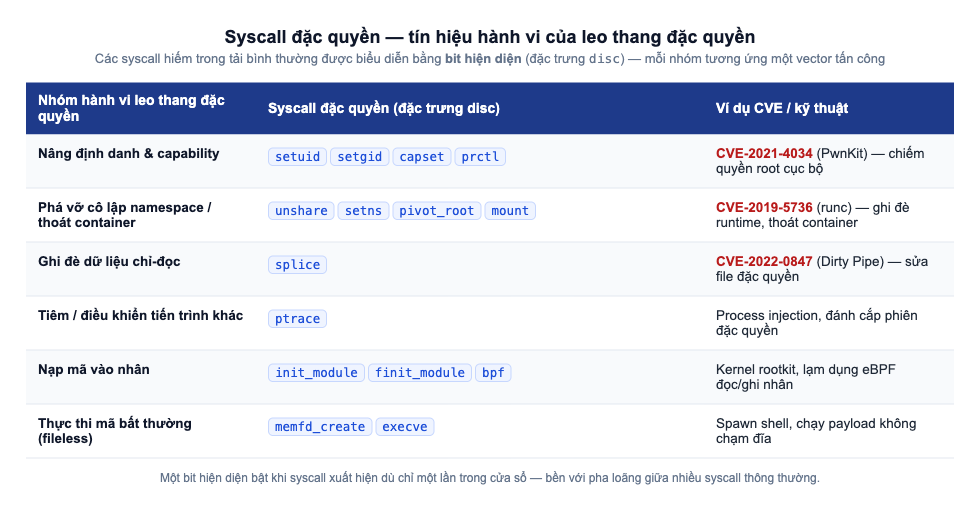
\includegraphics[width=\linewidth]{figures/privesc-syscalls}
  \caption{Ánh xạ các syscall đặc quyền (đặc trưng \texttt{disc}) sang nhóm hành vi
           leo thang đặc quyền và ví dụ CVE thực. Mỗi nhóm là một vector tấn công
           vượt ranh giới tenant; bit hiện diện của một syscall đặc quyền là tín
           hiệu phát hiện cốt lõi của cơ chế.}
  \label{fig:privesc}
\end{figure}

\subsection{Mô hình SyscallAD}
\begin{itemize}[leftmargin=1.6em]
  \item \textbf{VAE}~\cite{vae_kingma}: \texttt{hidden\_dim}=32, \texttt{latent\_dim}=8,
        huấn luyện \emph{chỉ} trên cửa sổ bình thường; điểm bất thường là lỗi tái
        cấu trúc. Huấn luyện đa hạt giống (seed 0,1,2), giữ hạt giống có AUC kiểm
        định tốt nhất để xử lý hiện tượng \emph{sụp đổ hậu nghiệm} (posterior
        collapse).
  \item \textbf{iForest}~\cite{iforest_liu}: 300 cây, \texttt{contamination}=0{,}02,
        cũng huấn luyện trên dữ liệu bình thường.
  \item \textbf{Hợp nhất tập hợp:}
        $s = 0{,}7\cdot\mathrm{RobustScale}(s_\text{VAE}) + 0{,}3\cdot\mathrm{RobustScale}(s_\text{iForest})$.
\end{itemize}

\subsection{Chọn ngưỡng (không rò rỉ)}
Ngưỡng phát hiện được chọn \emph{chỉ} trên tập kiểm định và lưu vào
\texttt{results.json}; tập kiểm tra không tham gia chọn ngưỡng. Khi phục vụ trực
tiếp, ngưỡng vận hành được hiệu chỉnh lại theo phân phối điểm quan sát trên cụm
(xem Mục~\ref{sec:evaluation}).

\subsection{Mở rộng: bộ phát hiện trực tiếp}
Thành phần suy luận đọc luồng sự kiện syscall từ Tetragon~\cite{tetragon} qua gRPC,
gom theo tiến trình, cắt cửa sổ $(15,3)$ và trích \emph{đúng} véc-tơ 43 chiều như
lúc huấn luyện (được kiểm tra ngang hàng bằng \texttt{tests/test\_feature\_parity.py}),
rồi chấm điểm bằng các mô hình đã lưu. Cảnh báo và chỉ số được phơi bày qua
Prometheus và trực quan hóa trên Grafana; nhật ký sự kiện Tetragon được thu thập
qua Loki/Promtail. Toàn bộ chạy bằng Docker/Kubernetes, không cài công cụ trực
tiếp lên máy chủ.
